\documentclass[preprint,12pt, a4paper, dvipsnames]{elsarticle}

\usepackage{amsmath,amssymb,amsthm}
\usepackage{caption}
\usepackage{float}
\usepackage{lineno}
\usepackage{listings}
\usepackage{mathtools}
\usepackage{subcaption}
\usepackage{todonotes}
\usepackage{url}
\usepackage{xcolor}

\definecolor{codegreen}{rgb}{0.25,0.93,0.31}
\definecolor{codegray}{rgb}{0.5,0.5,0.5}
\definecolor{codepurple}{rgb}{0.58,0,0.82}
\definecolor{backcolour}{rgb}{0.95,0.95,0.92}

\lstset{frame=tb,
	language=Python,
	aboveskip=3mm,
	belowskip=3mm,
	showstringspaces=false,
	columns=flexible,
	basicstyle={\small\ttfamily},
	breaklines=true,
	breakatwhitespace=true,
	tabsize=3,
	escapeinside={@}{@},
}
\restylefloat{table}

\newcommand{\eg}{{\emph{e.g.\/}}}
\newcommand{\ie}{{\emph{i.e.\/}}}
\newcommand{\ket}[1]{\ensuremath{|#1\rangle}}
\newcommand{\bra}[1]{\ensuremath{\langle#1|}}
\newcommand{\ketbra}[2]{\ensuremath{\ket{#1}\bra{#2}}}
\newcommand{\proj}[1]{\ensuremath{\ketbra{#1}{#1}}}
\newcommand{\braket}[2]{\ensuremath{\langle{#1}|{#2}\rangle}}
\newcommand{\floor}[1]{\ensuremath{\lfloor #1 \rfloor}}
\newcommand{\complexity}[1]{\ensuremath{\mathbf{#1}}}
\newcommand{\new}[1]{ \textcolor{red}{#1} }
\newcommand{\1}{{\rm 1\hspace{-0.9mm}l}}
\newcommand{\Id}{{\rm 1\hspace{-0.9mm}l}}
\newcommand{\connected}{\sim}
\newcommand{\SPAN}{\mathrm{span}}
\newcommand{\Lrm}{\ensuremath{\mathrm{L}}}
\newcommand{\Urm}{\ensuremath{\mathrm{U}}}
\newcommand{\ee}{\ensuremath{\mathrm{e}}}
\newcommand{\dd}{\ensuremath{\mathrm{d}}}
\newcommand{\ii}{\ensuremath{\mathrm{i}}}
\newcommand{\EE}{\mathcal{E}}
\newcommand{\XX}{\mathcal{X}}
\newcommand{\MM}{\mathcal{M}}
\newcommand{\NN}{\mathcal{N}}
\newcommand{\DD}{\mathcal{D}}
\newcommand{\TT}{\mathcal{T}}
\newcommand{\PP}{\mathcal{P}}
\newcommand{\QQ}{\mathcal{Q}}
\renewcommand{\SS}{\mathcal{S}}
\newcommand{\UU}{\mathcal{U}}
\newcommand{\HH}{\mathcal{H}}
\newcommand{\DU}{\mathcal{DU}}
\newcommand{\NOT}{\sigma_x}
\newcommand{\idop}[1][\XX]{\ensuremath{\1_{#1}}}
\newcommand{\diaguni}{\ensuremath{\mathcal{DU}}}
\newcommand{\diag}{\mathrm{diag}}
\newcommand{\tr}{\mathrm{tr}}
\newcommand{\textapprox}{\raisebox{0.5ex}{\texttildelow}}
\journal{SoftwareX}

\newtheorem{theorem}{Theorem}
\newtheorem{proposition}{Proposition}
\newtheorem{remark}{Remark}
\newtheorem{lemma}{Lemma}
\theoremstyle{definition}
\newtheorem{scheme}{Scheme}

\usepackage{xr}
\externaldocument{supplemental}

\begin{document}

\begin{frontmatter}

\title{PyQBench: a Python library for benchmarking gate-based quantum computers}

\author{Konrad Jałowiecki\corref{cor1}}
\ead{dexter2206@gmail.com}
\cortext[cor1]{Corresponding author}

\author{Paulina Lewandowska}
\author{\L ukasz Pawela}

\address{Institute of Theoretical and Applied Informatics, Polish Academy
	of Sciences, Ba{\l}tycka~5, 44-100 Gliwice, Poland}

\begin{abstract}

We introduce PyQBench, an innovative open-source framework for benchmarking gate-based quantum
computers. PyQBench can benchmark NISQ devices by verifying their capability of discriminating
between two von Neumann measurements. PyQBench offers a simplified, ready-to-use, command line
interface (CLI) for running benchmarks using a predefined family of measurements. For more advanced
scenarios, PyQBench offers a way of employing user-defined measurements instead of predefined ones.

\end{abstract}

\begin{keyword}
Quantum computing \sep
Benchmarking quantum computers \sep
Discrimination of quantum measurements \sep
Discrimination of von Neumann measurements \sep
Open-source \sep
Python programming

\PACS 03.67.-a \sep 03.67.Lx

\MSC 81P68

\end{keyword}

\end{frontmatter}

\section*{Current code version}
\label{}

\begin{table}[H]
\begin{tabular}{|l|p{5.5cm}|p{7.5cm}|}
\hline
C1 & Current code version & 0.1.1 \\
\hline
C2 & Permanent link to code/repository used for this code version & \url{https://github.com/iitis/PyQBench} \\
\hline
C3 & Code Ocean compute capsule & \texttt{https://codeocean.com/capsule/ 89088992-9a27-4712-8525-} \texttt{d92a9b23060f/tree}\\
\hline
C4 & Legal Code License & Apache License 2.0\\
\hline
C5 & Code versioning system used & git \\
\hline
C6 & Software code languages, tools, and services used & Python, Qiskit, AWS Braket \\
\hline
C7 & Compilation requirements, operating environments \& dependencies &
\texttt{Python >= 3.8}\newline
\texttt{numpy \textapprox= 1.22.0}\newline
\texttt{scipy \textapprox= 1.7.0}\newline
\texttt{pandas \textapprox= 1.5.0}\newline
\texttt{amazon-braket-sdk >= 1.11.1}\newline
\texttt{pydantic \textapprox= 1.9.1}\newline
\texttt{qiskit \textapprox= 0.37.2}\newline
\texttt{mthree \textapprox= 1.1.0}\newline
\texttt{tqdm \textapprox= 4.64.1}\newline
\texttt{pyyaml \textapprox= 6.0}\newline
\texttt{qiskit-braket-provider \textapprox= 0.0.3}\\
\hline
C8 & If available Link to developer documentation/manual &
\url{https://pyqbench.readthedocs.io/en/latest/}\\
\hline
C9 & Support email for questions & \url{dexter2206@gmail.com}\\
\hline
\end{tabular}
\caption{Code metadata}
\label{}
\end{table}


\linenumbers

\section{Motivation and significance}

Noisy Intermediate-Scale Quantum (NISQ)~\cite{preskill} devices are storming the market, with a wide
selection of devices based on different architectures and accompanying software solutions. Among
hardware providers offering public access to their gate--based devices, one could mention Rigetti
\cite{rigetti}, IBM \cite{ibmq}, Oxford Quantum Group \cite{oxforf}, IonQ \cite{ionq} or Xanadu
\cite{xanadu}. Other vendors offer devices operating in different paradigms. Notably, one could
mention D-Wave \cite{dwave} and their quantum annealers, or QuEra devices \cite{quera} based on
neural atoms. Most vendors provide their own software stack and application programming interface
for accessing their devices. To name a few, Rigetti's computers are available through their Forest
SDK \cite{sdk} and PyQuil library \cite{pyquil} and IBM Q \cite{ibmq} computers can be accessed
through Qiskit \cite{qiskit} or IBM Quantum Experience web interface \cite{ibmqplatform}. Some cloud
services, like Amazon Braket \cite{amazon}, offer access to several quantum devices under a unified
API. On top of that, several libraries and frameworks can integrate with multiple hardware vendors.
Examples of such frameworks include IBM Q's Qiskit or Zapata Computing's Orquestra \cite{zapata}.

It is well known that NISQ devices have their limitations \cite{preskillnew}. The question is to
what extent those devices can perform meaningful computations? To answer this question, one has to
devise a methodology for benchmarking them. For gate--based computers, on which this paper focuses,
there already exist several approaches. One could mention randomized benchmarking
\cite{liu2022sampling, knill2008randomized, wallman2014randomized, helsen2022general,
cornelissen2021scalable}, benchmarks based on the quantum volume \cite{cross2019validating,
moll2018quantum, pelofske2022volume}.

In this paper, we introduce a different approach to benchmarking gate--based devices with a simple
operational interpretation. In our method, we test how well the given device is at guessing which of
the two known von Neumann measurements were performed during the experiment. We implemented our
approach in an open-source Python library called PyQBench. The library supports any device available
through the Qiskit library, and thus can be used with providers such as IBM Q or Amazon Braket.
Along with the library, the PyQBench package contains a command line tool for running most common
benchmarking scenarios.

\section{Existing benchmarking methodologies and software}
Unsurprisingly, PyQBench is not the only software package for benchmarking gate--based devices.
While we believe that our approach has significant benefits over other benchmarking techniques, for
completeness, in this section we discuss some of the currently available similar software.

Probably the simplest benchmarking method one could devise is simply running known algorithms and
comparing outputs with the expected ones. Analyzing the frequency of the correct outputs, or the
deviation between actual and expected outputs distribution provides then a metric of the performance
of a given device. Libraries such as Munich Quantum Toolkit (MQT) \cite{mqt2022, mqt-bench} or
SupermarQ \cite{supermarq, supermarkq-github} contain benchmarks leveraging multiple algorithms,
such as Shor's algorithm or Grover's algorithm.
% or  implementing e.g. GHZ state \cite{ghz}.
Despite being intuitive and easily interpretable, such benchmarks may have some problems. Most
importantly, they assess the usefulness of a quantum device only for a very particular algorithm,
and it might be hard to extrapolate their results to other algorithms and applications. For
instance, the inability of a device to consistently find factorizations using Shor's algorithms does
not tell anything about its usefulness in Variational Quantum Algorithm's.

Another possible approach to benchmarking quantum computers is randomized benchmarking. In this
approach, one samples circuits to be run from some predefined set of gates (e.g. from the Clifford
group) and tests how much the output distribution obtained from the device running these circuits
differs from the ideal one. It is also common to concatenate randomly chosen circuits with their
inverses (which should yield the identity circuit) and run those concatenated circuits on the
device. Libraries implementing this approach include Qiskit \cite{qiskit-randomized} or PyQuil
\cite{forest-benchmarking}.

Another quantity used for benchmarking NISQ devices is quantum volume. The quantum volume
characterizes capacity of a device for solving computational problems. It takes into account
multiple factors like number of qubits, connectivity and measurement errors. The Qiskit library
allows one to measure quantum volume of a device by using its \texttt{qiskit.ignis.verifica \\
tion.quantum\_volume}. Other implementations of Quantum Volume can be found as well, see e.g.
\cite{volume-in-practice}.

Finally, we should mention cross-entropy
benchmarking~\cite{boixo2018characterizing}, which was utlilized in validation
of the Sycamore-53 QPU supremacy experiments~\cite{arute2019quantum}. In this
approach, the quality of an algorithm implemented on the QPU is measured by
calculating the cross entropy of bit-strings actually sampled from the QPU,
compared to ideal bitstrings.

\section{Preliminaries and discrimination scheme approach}

In this section, we describe how the benchmarking process in PyQBench works. We start by
discussing necessary mathematical preliminaries. Then, we present the general form of the
discrimination scheme used in PyQBench and practical considerations on how to implement it taking
into account the limitations of the current NISQ devices. We encourage the readers interested
in a more in--depth discussion of the mathematical foundations behind our discrimination scheme to read
Section \ref{app:preliminaries} in the supplemental materials.

\subsection{Von Neumann Measurements}\label{sec:maths}

A von Neumann measurement $\PP$ is a collection of rank--one projectors
$\{\proj{u_0}, \ldots, \proj{u_{d-1}}\}$, called effects, that sum up to the identity operator, i.e.
$ \, \, \sum_{i=0}^{d-1} \proj{u_i} = \1$. If $U$ is a unitary matrix of size $d$, one can construct
a von Neumann measurement $\PP_{U}$ by taking projectors onto its columns. In this case we say that
$\PP_{U}$ is described by the matrix $U$.

Typically, NISQ devices can only perform measurements in computational $Z$-basis, i.e. $U=\1$. To
implement an arbitrary von Neumann measurement $\PP_{U}$, one has to first apply $U^\dagger$ to the
measured system and then follow with $Z$-basis measurement. This process, depicted in Fig.
\ref{fig:vonneumann}, can be viewed as performing a change of basis in which measurement is
performed prior to measurement in the computational basis.

\begin{figure}[h!]
	\centering
	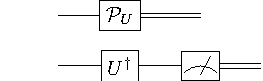
\includegraphics[scale=1.7]{pics/vonneuman}
	\caption{Implementation of a von Neumann measurement using measurement in computational basis.
	The upper circuit shows a symbolic representation of a von Neumann measurement $\PP_{U}$. The
	bottom, equivalent circuit depicts its decomposition into a change of basis followed
	by measurement in the $Z$ basis.}
	\label{fig:vonneumann}
\end{figure}

\subsection{Discrimination scheme}\label{sec:discrimination-scheme}

Benchmarks in PyQBench work by experimentally determining the probability of correct discrimination
between two von Neumann measurements by the device under test and comparing the result with the
ideal, theoretical predictions.

Without loss of generality\footnote{Explaining why we can consider only discrimination scheme
between $\PP_{\Id}$ and $\PP_{U}$ is beyond the scope of this paper. See
\cite{puchala2018strategies} for a in depth explanation.}, we consider discrimination task between
single qubit measurements $\PP_\Id$, performed in the computational Z-basis, and an alternative
measurement $\PP_U$ performed in the basis $U$. 
The discrimination scheme presented in Fig.~\ref{fig:theoretical_scheme} requires an
auxiliary qubit. First, the joint system is prepared in some state $\ket{\psi_0}$. Then, one of the
measurements, either $\PP_U$ or $\PP_\1$, is performed on the first part of the system. Based on its
outcome $i$, we choose another binary measurement $\mathcal{P}_{V_i}$ and perform it on the second qubit,
obtaining the outcome $j$. Finally, if $j=0$, we say that the performed measurement is
$\mathcal{P}_U$, otherwise we say that it was $\mathcal{P}_\Id$. 

Note, however, that the discrimination scheme described above can work regardless of dimensionality 
of the unitary $U$. The main difference is the dimension of the auxiliary system, which in general
can be larger than two. This dimension depends on the Schmidt rank of the optimal input state. However, 
for most discrimination schemes, the  Schmidt rank equals at most two, and hence the auxiliary system
is also a qubit, see \cite{puchala2018strategies} for details. Note that the final measurement $\PP_{V_i}$ 
is always binary, independently of the dimension of auxiliary system.

Naturally, we need to repeat the
same procedure multiple times for both measurements to obtain a reliable estimate of the underlying
probability distribution. In PyQBench, we assume that the experiment is repeated the same number of
times for both $\PP_U$ and $\PP_\Id$.

In principle, our discrimination scheme could be used with any choice of
$\ket{\psi_0}$ and final measurements $\PP_{V_i}$. However, we argue that it is best to choose those
components so that they maximize the probability of correct discrimination. To see that,
suppose that some choice of $\ket{\psi_0}, \PP_{V_0}, \PP_{V_1}$ allows for correctly discriminating
between two measurements with probability equal to one, i.e. on a perfect quantum computer you will always
make a correct guess. Then, on real hardware, we might obtain any empirical value in range $\left[\frac{1}{2},
1\right]$. On the other hand, if we choose the components of our scheme such that the successful
discrimination probability is $\frac{3}{5}$, the possible range of empirically obtainable probabilities
is only $\left[\frac{1}{2}, \frac{3}{5}\right]$. Hence, in the second case, the discrepancy between theoretical and empirical
results will be less pronounced.


\begin{figure}[h!]
	\centering
	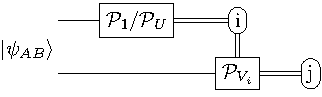
\includegraphics[scale=1.7]{pics/theoretical_scheme}
	\caption{Theoretical  scheme of discrimination  between von Neumann measurements $\PP_{U}$ and $\PP_\Id$. }
	\label{fig:theoretical_scheme}
\end{figure}

\subsubsection{Implementation of discrimination scheme on actual NISQ devices}

Current NISQ devices are unable to perform conditional measurements, which is the biggest obstacle
to implementing our scheme on real hardware. However, we circumvent this problem by slightly
adjusting our scheme so that it only uses components available on current devices. For this purpose,
we use two possible options: using a postselection or a direct sum $V_0^\dagger\oplus V_1^\dagger$.

\begin{scheme}(Postselection)

	The first idea uses a postselection scheme. In the original scheme, we measure the first qubit
	and only then determine which measurement should be performed on the second one. Instead of doing
	this choice, we can run two circuits, one with $\PP_{V_0}$ and one with $\PP_{V_1}$ and measure both
	qubits. We then discard the results of the circuit for which label $i$ does not match measurement
	label $k$. Hence, the circuit for postselection looks as depicted in Fig.
	\ref{fig:postselection}.

	\begin{figure}[h!]
		\centering
		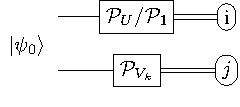
\includegraphics[scale=1.7]{pics/postselection_no_channels}

		\caption{
			A schematic representation of the setup for distinguishing
			measurements $\PP_{U}$ and $\PP_{\Id}$ using postselection approach.
			In postselection scheme, one runs such circuits for both $k=0,1$ and discards results
			for cases when there is a mismatch between $k$ and $i$.
		}\label{fig:postselection}
	\end{figure}

	To perform the benchmark, one needs to run multiple copies of the postselection circuit,
	with both $\PP_U$ and $\PP_\1$. Each circuit has to be run in both variants, one with final
	measurement $\PP_{V_0}$ and the second with the final measurement $\PP_{V_1}$.
	The experiments can thus be grouped into classes identified by tuples of the form
	$(\mathcal{Q}, k, i, j)$, where $\mathcal{Q} \in \{\PP_U, \PP_\Id\}$ denotes the chosen
	measurement, $k \in \{0,1\}$ designates the final measurement used, and $i \in \{0,1\}$ and $j
	\in \{0,1\}$ being the labels of outcomes as presented in Fig. \ref{fig:postselection}.
	We then discard all the experiments for which $i \ne k$. The total number of valid experiments
	is thus:

	\begin{equation}
	N_\text{total} = \#\{(\QQ, k, i, j): k = i \}.
	\end{equation}

	Finally, we count the valid experiments resulting in successful discrimination.
	If we have chosen $\PP_U$, then we guess correctly iff $j=0$. Similarly, for
	$P_\Id$, we guess correctly iff $j=1$. If we define
	\begin{eqnarray}
	N_{\PP_U} &= \#\{(\mathcal{Q}, k, i, j): \mathcal{Q} = \PP_U, k = i, j = 0\}, \\
	N_{\PP_\Id} &= \#\{(\mathcal{Q}, k, i, j): \mathcal{Q} = \PP_\Id, k = i, j = 1\},
	\end{eqnarray}
	then the empirical success probability can be computed as

	\begin{equation}
	p_{\text{succ}}(\PP_{U}, \PP_{\Id}) = \frac{N_{\PP_U} + N_{\PP_\Id}}{N_{\text{total}}}.
	\end{equation}
	The $p_{\text{succ}}$ is the quantity reported to the user as the result of the benchmark.
\end{scheme}

\begin{scheme}(Direct sum)

The second idea uses the direct sum $V_0^\dagger \oplus V_1^\dagger$ implementation. Here, instead
of performing a conditional measurement $\PP_{V_k}$, where $k\in \{0,1\}$,  we run circuits
presented in Fig.~\ref{fig:controlled}.
	\begin{figure}[h!]
		\centering
		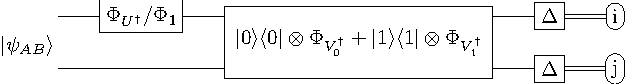
\includegraphics[width=0.8\textwidth]{pics/controlled_unitary}

		\caption{ A schematic representation of the setup for distinguishing
			measurements $\PP_{U}$ and $\PP_{\Id}$ using the $V_0^\dagger \oplus V_1^\dagger$ direct sum.
		}\label{fig:controlled}
	\end{figure}

	One can see why such a circuit is equivalent to the original discrimination scheme.
	If we rewrite the block-diagonal matrix $V_0^\dagger \oplus V_1^\dagger$ as follows:
	\begin{equation}
		\label{eq:directsum}
		V_0^\dagger \oplus V_1^\dagger = \proj{0}\otimes V_0^\dagger + \proj{1} \otimes V_1^\dagger,
	\end{equation}
	we can see that the direct sum in Eq. \eqref{eq:directsum} commutes with the measurement on the
	first qubit. Thanks to this, we can switch the order of operations to obtain the circuit from
	Fig. \ref{fig:directsum}. Now, depending on the outcome $i$, one of the summands in
	Eq. \eqref{eq:directsum} vanishes, and we end up performing exactly the same operations as in
	the original scheme.

	\begin{figure}[h!]
		\centering
		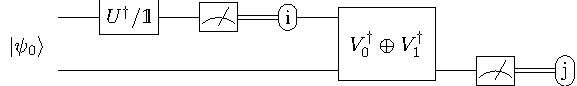
\includegraphics[width=\textwidth]{pics/direct_sum}
		\caption{Rewritten representation of the setup for distinguishing
		measurements $\PP_{U}$ and $\PP_{\Id}$ using the $V_0^\dagger \oplus V_1^\dagger$ direct
		sum.
		}\label{fig:directsum}
	\end{figure}

	In this scheme, the experiment can be characterized by a pair $(\mathcal{Q}, i,j)$, where
	$\mathcal{Q} = \{ \PP_{U}, \PP_{\Id} \}$ and $i,j \in \{0,1\}$ are the output labels. The number
	of successful trials for $U$ and $\Id$, respectively, can be written  as
	\begin{eqnarray}
	N_{\PP_U} &= \#\{(\mathcal{Q},  i, j): \mathcal{Q} = \PP_U, j = 0\}, \\
	N_{\PP_\Id} &= \#\{(\mathcal{Q},  i, j): \mathcal{Q} = \PP_\Id, j = 1\}.
	\end{eqnarray}
	Then, the probability of correct discrimination between $\PP_{U} $ and $\PP_\Id$ is given by
	\begin{equation}
	p_{\text{succ}} = \frac{N_{\PP_{U}} + N_{\PP_{\Id}}}{N_{\text{total}}},
	\end{equation}
	where $N_{\text{total}}$ is the number of trials.
\end{scheme}

Compared to these approaches, our approach allows for a very simple operational
interpretation of the scheme and its results. This is especially useful for
newcomers to the field, who may be put off by more complicated approaches.
Another benefit is, especially for advanced users, the ability to control
resources utilized during the benchmarking. We can consider here resources such
as entanglement or coherence. Finally, the figure of merit we wish to calculate and
to which we compare the results is fairly simple to obtain. The main downside of
our approach is the exponential number of circuits we need to consider.

% \subsubsection{Constructing optimal discrimination scheme}
% To construct the optimal discrimination scheme, one starts by calculating the probability of correct discrimination. Using the celebrated result by Helstrom~\cite{helstrom1976quantum}, one finds that the  optimal probability of correct discrimination between two quantum measurements, $\PP$  and $\mathcal{Q}$, is
% \begin{equation}
% p_{\text{succ}}(\PP, \mathcal{Q}) =  \frac12 + \frac14 \| \PP - \mathcal{Q} \|_\diamond,
% \end{equation}
% where
% \begin{equation}
% \|\PP - \QQ\|_\diamond = \max_{\| \ket{\psi}\|_1=1} \| \left( (\PP - \QQ) \otimes \1\right) (\proj{\psi}) \|_1.
% \end{equation}
% The quantum state $\ket{\psi_0}$ maximizing the diamond norm above is called the
% \emph{discriminator}, and can be computed e.g. using semidefinite programming (SDP)
% \cite{watrous,watrous2021simplier}. Furthermore,  using the proof of the Holevo-Helstrom theorem, it is
% possible to construct corresponding unitaries $V_0$, $V_1$ to create the optimal
% discrimination strategy. For brevity, we do not describe this procedure here. Instead, we refer the
% interested reader to \cite{watrous}.

 \section{Software description}
 \label{}
 This section is divided into two parts.
 In Section~\ref{sec:sortware-functionalities} we describe functionalities of PyQBench
 package. Next, in Section~\ref{sec:sortware-architecture}, we give a general overview of the
 software architecture.

\subsection{Software Functionalities}\label{sec:sortware-functionalities}

The PyQBench can be used in two modes: as a Python library and as a CLI script. When used as a
library, PyQBench allows the customization of discrimination scheme. The user provides
a unitary matrix $U$ defining the measurement to be discriminated, the discriminator $\ket{\psi_0}$,
and unitaries $V_0$ and $V_1$ describing the final measurement. The PyQBench library provides then
the following functionalities.

\begin{enumerate}
	\item Assembling circuits for both postselection and direct sum--based discrimination schemes.
	\item Executing the whole benchmarking scenario on specified backend (either real hardware or
	software simulator).
	\item Interpreting the obtained outputs in terms of discrimination probabilities.
\end{enumerate}
Note that the execution of circuits by PyQBench is optional. Instead, the user might want to opt in
for fine-grained control over the execution of the circuits. For instance, suppose the user wants to
simulate the discrimination experiment on a noisy simulator. In such a case, they can define the
necessary components and assemble the circuits using PyQBench. The circuits can then be altered,
e.g. to add noise to particular gates, and then run using any Qiskit backend by the user. Finally,
PyQBench can be used to interpret the measurements to obtain discrimination probability.

The PyQBench library also contains a readily available implementation of all necessary components
needed to run discrimination experiments for parametrized Fourier family of measurements (see
Section \ref{app:optimal-probability} in supplemental material). However, if one only wishes to use
this particular family of measurements in their benchmarks, then using PyQBench as a command line tool
might be more straightforward. PyQBench's command line interface allows running the benchmarking process
without writing Python code. The configuration of CLI is done by YAML \cite{yaml} files describing the
benchmark to be performed and the description of the backend on which the benchmark should be run.
The same benchmark can be used with different backends and vice versa.

\subsection{Software Architecture}\label{sec:sortware-architecture}

\subsubsection{Overview of the software structure}
As already described, PyQBench can be used both as a library and a CLI. Both functionalities are
implemented as a part of \texttt{qbench} Python package. The exposed CLI tool is also named
\texttt{qbench}. For brevity, we do not discuss the exact structure of the package here, and instead
refer an interested reader to the source code available at GitHub \cite{pyqbenchgithub} or at the
reference manual \cite{pyqbenchdocs}.

PyQBench can be installed from official Python Package Index (PyPI) by running \texttt{pip install
pyqbench}. In a properly configured Python environment the installation process should also make the
\texttt{qbench} command available to the user without a need for further configuration.

\subsubsection{Integration with hardware providers and software simulators}

PyQBench is built around the Qiskit \cite{qiskit} ecosystem. Hence, both the CLI tool and the
\texttt{qbench} library can use any Qiskit--compatible backend. This includes, IBM Q backends
(available by default in Qiskit) and Amazon Braket devices and simulators (available through
\texttt{qiskit-braket-provider} package \cite{qiskit-braket-provider,
qiskit-braket-provider-github}).

When using PyQBench as library, instances of Qiskit backends can be passed to functions that expect
them as parameters. However, in CLI mode, the user has to provide a YAML file describing the
backend. An example of such file can be found in Section \ref{sec:examples}, and the detailed
description of the expected format can be found at PyQBench's documentation.

\subsubsection{Command Line Interface}
\label{sec:cli}

The Command Line Interface (CLI) of PyQBench has nested structure. The general form of the CLI
invocation is shown in listing \ref{lst:cli}.
\begin{lstlisting}[caption=Invocation of \texttt{qbench} script, label=lst:cli]
qbench <benchmark-type> <command> <parameters>
\end{lstlisting}
Currently, PyQBench's CLI supports only one type of benchmark (discrimination of parametrized
Fourier family of measurements), but we decided on hierarchically structuring the CL to allow for
future extensions. Thus, the only accepted value of \texttt{<benchmark-type>} is
\texttt{disc-fourier}.
%
The \texttt{qbench disc-fourier} command has four subcommands:

\begin{itemize}
	\item \texttt{benchmark}: run benchmarks. This creates either a result YAML file containing the
		measurements or an intermediate YAML file for asynchronous experiments.
	\item \texttt{status}: query status of experiments submitted for given benchmark. This command
		is only valid for asynchronous experiments.
	\item \texttt{resolve}: query the results of asynchronously submitted experiments and write the
		result YAML file. The output of this command is almost identical to the result obtained from
		synchronous experiments.
	\item \texttt{tabulate}: interpret the results of a benchmark and summarize them in the CSV
	file.
\end{itemize}
%
We present usage of each of the above commands later in section \ref{sec:examples}.

\subsubsection{Asynchronous vs. synchronous execution}
PyQBench's CLI can be used in synchronous and asynchronous modes. The mode of execution is defined
in the YAML file describing the backend (see Section \ref{sec:examples} for an example of this
configuration). We decided to couple the mode of execution to the backend description because some
backends cannot work in asynchronous mode.

When running \texttt{qbench disc-fourier benchmark} in asynchronous mode, the PyQBench submits all
the circuits needed to perform a benchmark and then writes an intermediate YAML file containing
metadata of submitted experiments. In particular, this metadata contains information on correlating
submitted job identifiers with particular circuits. The intermediate file can be used to query the
status of the submitted jobs or to resolve them, i.e. to wait for their completion and get the
measurement outcomes.

In synchronous mode, PyQBench first submits all jobs required to run the benchmark and then
immediately waits for their completion. The advantage of this approach is that no separate
invocation of \texttt{qbench} command is needed to actually download the measurement outcomes. The
downside, however, is that if the script is interrupted while the command is running, the
intermediate results will be lost. Therefore, we recommend using asynchronous mode whenever
possible.

\section{Illustrative examples}
\label{sec:examples} In this section, we demonstrate the usage of PyQBench.
For brevity, we decided to present only the usage of the CLI tool, as it is likely to be the most
popular use case. We refer readers interested in implementing their discrimination schemes using
custom measurements to PyQBench's documentation \cite{pyqbenchdocs}, where we describe the whole
process, and to the Section \ref{app:hadamard} in the supplemental material, where we discuss
the relevant mathematical details.

\subsection{Using \texttt{qbench} CLI}
PyQBench offers a simplified way of conducting benchmarks using a Command Line Interface (CLI).
The workflow with PyQBench's CLI can be summarized as the following list of steps:

\begin{enumerate}
  \item Preparing configuration files describing the backend and the experiment scenario.
  \item Submitting/running experiments. Depending on the experiment scenario, execution can be
		synchronous, or asynchronous.
  \item (optional) Checking the status of the submitted jobs if the execution is asynchronous.
  \item Resolving asynchronous jobs into the actual measurement outcomes.
  \item Converting obtained measurement outcomes into tabulated form.
\end{enumerate}
\subsubsection{Preparing configuration files}
The configuration of PyQBench CLI is driven by YAML files. The first configuration file describes
the experiment scenario to be executed. The second file describes the backend. Typically, this
backend will correspond to the physical device to be benchmarked, but for testing purposes, one
might as well use any other Qiskit--compatible backend including simulators. Let us first describe
the experiment configuration file, which might look as follow.
\begin{lstlisting}[language=Python, caption=Defining the experiment, label=lst:experiment]
type: discrimination-fourier
qubits:
	- target: 0
	  ancilla: 1
	- target: 1
      ancilla: 2
angles:
	start: 0
	stop: 2 * pi
	num_steps: 3
gateset: ibmq
method: direct_sum
num_shots: 100
\end{lstlisting}

The second configuration file describes the backend. We decided to decouple the experiment and the
backend files because it facilitates their reuse. For instance, the same experiment file can be used
to run benchmarks on multiple backends, and the same backend description file can be used with
multiple experiments.

Different Qiskit backends typically require different data for their initialization. Hence, there
are multiple possible formats of the backend configuration files understood by PyQBench. We refer
the interested reader to the PyQBench's documentation. Below we describe an example YAML file
describing IBM Q backend named Quito.
\begin{lstlisting}[language=Python, caption=IBMQ backend, label=lst:backend]
name: ibmq_quito
asynchronous: false
provider:
	hub: ibm-q
	group: open
	project: main
\end{lstlisting}
IBMQ backends typically require an access token to IBM Quantum Experience. Since it would be unsafe
to store it in plain text, the token has to be configured separately in \texttt{IBMQ\_TOKEN}
environmental variable.

\subsubsection{Running the experiment and collecting measurements data}
After preparing YAML files defining experiment and backend,
running the benchmark can be launched by using the following command line invocation:
\begin{lstlisting}[language=Python]
qbench disc-fourier benchmark experiment_file.yml backend_file.yml
\end{lstlisting}
The output file will be printed to stdout. Optionally, the \texttt{- -output OUTPUT} parameter might
be provided to write the output to the \texttt{OUTPUT} file instead.
\begin{lstlisting}[language=Python]
qbench disc-fourier benchmark experiment_file.yml backend_file.yml --output async_results.yml
\end{lstlisting}
The result of running the above command can be twofold:
\begin{itemize}
	\item If the backend is asynchronous, the output will contain intermediate data containing, amongst
		others, \texttt{job\_ids} correlated with the circuit they correspond to.
	\item If the backend is synchronous, the output will contain measurement outcomes (bitstrings)
		for each of the circuits run.
\end{itemize}

For the synchronous experiment, the part of the output looks similar to the one below. The whole YAML
file can be seen in Section \ref{app:example.} in the supplemental material.
%Consider the particular experiment data
\begin{lstlisting}[language=Python]
data:
- target: 0
  ancilla: 1
  phi: 0.0
  results_per_circuit:
  - name: id
  histogram: {'00': 28, '01': 26, '10': 21, '11': 25}
  mitigation_info:
	target: {prob_meas0_prep1: 0.052200000000000024, prob_meas1_prep0: 0.0172}
	ancilla: {prob_meas0_prep1: 0.05900000000000005, prob_meas1_prep0: 0.0202}
  mitigated_histogram: {'00': 0.2637212373658018, '01': 0.25865061319892463, '10': 0.2067279352110304, '11': 0.2709002142242433}
\end{lstlisting}

\subsubsection{(Optional) Getting status of asynchronous jobs}
 PyQBench provides also a helper command that will fetch the statuses of asynchronous jobs. The command is:
\begin{lstlisting}[language=Python]
qbench disc-fourier status async_results.yml
\end{lstlisting}
and it will display dictionary with histogram of statuses.

\subsubsection{Resolving asynchronous jobs}
For asynchronous experiments, the stored intermediate data has to be resolved in actual
measurements' outcomes. The following command will wait until all jobs are completed and then write
a result file.
\begin{lstlisting}[language=Python]
qbench disc-fourier resolve async-results.yml resolved.yml
\end{lstlisting}
The resolved results, stored in \texttt{resolved.yml}, would look just like if the experiment was
run synchronously. Therefore, the final results will look the same no matter in which mode the
benchmark was run, and hence in both cases the final output file is suitable for being an input for
the command computing the discrimination probabilities.

\subsubsection{Computing probabilities}
As a last step in the processing workflow, the results file has to be passed to \texttt{tabulate}
command:
\begin{lstlisting}[language=Python]
qbench disc-fourier tabulate results.yml results.csv
\end{lstlisting}
A sample CSV file is provided in Table \ref{fig:tabulateresults}.
\begin{table}[ht!]
\begin{center}
	\begin{tabular}{|c c c c c c|} 
		\hline
		target & ancilla & phi & ideal$\_$prob  & disc$\_$prob & mit$\_$disc$\_$prob \\ [0.5ex] 
		\hline\hline
		0 & 1 & 0 & 0.5 & 0.46 & 0.45  \\ 
		\hline
		0 & 1 & 3.14 & 1 & 0.95 & 0.98  \\
		\hline
		0 & 1 & 6.28 & 0.5 & 0.57 & 0.58  \\
		\hline
		1 & 2 & 0 & 0.5  & 0.57 & 0.57 \\
		\hline
		1 & 2 & 3.14 & 1 & 0.88 & 0.94  \\ 
		\hline
		1 & 2 & 6.28 & 0.5 & 0.55 & 0.56  \\ 
		\hline
	\end{tabular}
\caption{The resulting CSV file contains table with columns \texttt{target}, \texttt{ancilla}, \texttt{phi},
	\texttt{ideal\_prob}, \texttt{disc\_prob} and, optionally, \texttt{mit\_disc\_prob}. Each row in the
	table describes results for a tuple of \texttt{(target, ancilla, phi)}.  The reference optimal value
	of discrimination probability is present in \texttt{ideal\_prob} column, whereas the obtained,
	empirical discrimination probability can be found in the \texttt{disc\_prob} column. The
	\texttt{mit\_disc\_prob} column contains empirical discrimination probability after applying the
	\texttt{Mthree} error mitigation \cite{mthree, mthreepublication}, if it was applied.}
\label{fig:tabulateresults}
\end{center}
\end{table}



\section{Impact}
With the surge of availability of quantum computing architectures in recent years it becomes
increasingly difficult to keep track of their relative performance. To make this case even more
difficult, various providers give access to different figures of merit for their architectures. Our
package allows the user to test various architectures, available through \texttt{qiskit} and Amazon
BraKet using problems with simple operational interpretation. We provide one example built-in in the
package. Furthermore, we provide a powerful tool for the users to extend the range of available
problems in a way that suits their needs.

Due to this possibility of extension, the users are able to test specific aspects of their
architecture of interest. For example, if their problem is related to the amount of coherence (the
sum of absolute value of off-diagonal elements) of the states present during computation, they are
able to quickly prepare a custom experiment, launch it on desired architectures, gather the result,
based on which they can decide which specific architecture they should use.

Finally, we provide the source code of PyQBench on GitHub~\cite{pyqbenchgithub} under an open source
license which will allow users to utilize and extend our package in their specific applications.

\section{Conclusions}
\label{}

In this paper, we presented a Python library PyQBench, an innovative open-source framework for
benchmarking gate-based quantum computers.
PyQBench can benchmark NISQ devices by verifying their capability of discriminating between two von
Neumann measurements. PyQBench offers a simplified, ready-to-use, command line interface (CLI) for
running benchmarks using a predefined parameterized Fourier family of measurements. For more
advanced scenarios, PyQBench offers a way of employing user-defined measurements instead of
predefined ones.

\section{Conflict of Interest}
We wish to confirm that there are no known conflicts of interest associated with this publication
and there has been no significant financial support for this work that could have influenced its
out- come.


\section*{Acknowledgements}

This work is supported by the project “Near-term quantum computers Challenges, optimal
implementations and applications” under Grant Number POIR.04.04.00-00-17C1/18-00, which is carried
out within the Team-Net programme of the Foundation for Polish Science co-financed by the European
Union under the European Regional Development Fund. PL is also a holder of European Union
scholarship through the European Social Fund, grant InterPOWER (POWR.03.05.00-00-Z305).

\bibliographystyle{unsrt}
\bibliography{references}
\end{document}
